\chapter{Diskussion}
\label{chap_disc}


Bei der Betrachtung aller Ergebnisse aus den RL Experimenten kann zunächst festgestellt werden, dass die Erweiterung des Schreiboperators zu einer Verbesserung der Ergebnisse führt. Darüber hinaus wirkt sich die Verwendung der GRU-basierten Schreiboperation positiv auf die Resultate aus, wenn die Aufgabenstellung schwieriger wird. Dies gilt sowohl für die Grundvariante der Neural Map als auch für die Variante mit der Erweiterung des Schreiboperators. Außerdem erzielen alle betrachteten Varianten der Neural Map bessere Ergebnisse als die Referenz, das LSTM. Lediglich im Rahmen des separaten Speichertests konnte anhand der dort verwendeten Bewertungskriterien kein Unterschied zwischen der Grundvariante und der Erweiterung festgestellt werden.

In Abschnitt XXX wurden die Ergebnisse zur detaillierten Analyse in drei Mengen eingeteilt.

Hierbei fällt auf, dass der optimale Weg in der Menge \glqq Ziel 2/3 besucht\grqq{} für alle Größen der verwendeten Umgebung signifikant geringer ist als in den beiden anderen Mengen. Darüber hinaus enthält diese Menge im Durchschnitt erheblich weniger Episoden als die anderen beiden. Um dafür einen Erklärungsansatz zu finden, wurden sich die Trajektorien diverser Episoden im Detail angeschaut. Dabei kann beobachtet werden, dass der Agent, wenn er ein Ziel beobachtet dieses in der Regel auch abläuft. Dies geschieht unabhängig davon, ob es sich um das richtige Ziel handelt oder nicht. In der kleinsten Umgebungsgröße passiert dieses Verhalten nahezu immer. Mit zunehmender Umgebungsgröße läuft der Agent auch einmal an einem Ziel, das bereits Teil seiner Observation ist vorbei. Auch dies geschieht unabhängig davon, um welches Ziel es sich handelt. Die Situation, dass er ein entsprechendes Folgeziel nur beobachtet und nicht abläuft, passiert nur, wenn er das entsprechende Folgeziel unmittelbar zusammen mit seinem eigentlich Ziel beobachtet.



Bei der Betrachtung der Trajektorien konnten noch weitere Auffälligkeiten im Verhalten des Agenten ausgemacht werden. Die Varianten mit der Erweiterung des Schreiboperators neigen stark dazu, sich zu Beginn der Episode auf der Stelle zu drehen. Dies stellt ein sehr effizientes Verhalten hinsichtlich der Erkundung dar, da auf diese Weise mit jeder Aktion die Observation maximal viele ungesehene Felder enthält. Dies ist in Abbildung XXX veranschaulicht. Würde der Agent zu Beginn der Episode einen Schritt nach vorne gehen, so würde die daraus resultierende Observation drei unbekannte Felder enthalten. Dreht er sich jedoch auf der Stelle, so erschließt er mit der ersten Drehung acht neue Felder, mit der zweiten Drehung sieben und mit der dritten Drehung sechs. Durch dieses Verhalten findet der entsprechende Agent Ziele die nah um seine Startposition liegen unabhängig von seiner initialen Blickrichtung. Es könnte sein, dass dieses Vehalten durch die Erweiterung des Schreiboperators begünstigt wird, da selbiger zumindest mit jeder Drehung auch eine neue Speicherposition beschreibt. Die Grundvarianten beschreiben bei der beschriebenen Drehung immer dieselbe Speicherstelle, da sich die Position des Agenten nicht verändert.



FWMG

Im Folgenden soll erklärt werden, warum die zusätzliche Schrittanzahl in den Mengen \glqq Ziel 2/3 besucht / gesehen\grqq{} immer geringer ist als in den Mengen \glqq Ziel 2/3 nie beobachtet\grqq{}. Auch dafür werden die Trajektorien genauer untersucht. Es fällt auf, dass alle Modelle zu Beginn der Episoden die vier Gänge in einer zufälligen Reihenfolge nach den Zielen absuchen. Während die Neural Map Varianten dabei fast nie einen Gang doppelt erkunden, passiert dies beim LSTM zwar auch nicht häufig aber schon öfter. Dies könnte ein Indiz dafür sein, dass die Karte der Neural Map bei der Exploration hilfreich ist.



Obwohl die ursprüngliche Einteilung in drei Mengen für diese Umgebung verworfen wurde, liegen die Einteilungen für drei Mengen dennoch vor. Dabei war insbesondere auffällig, dass bei drei Zielen die GRU-basierten Varianten mehrere Hundert Episoden in der Menge \glqq Ziel 2 gesehen\grqq{} hätten. Es gelingt diesen Varianten somit häufiger spätere Ziele nicht abzulaufen, sondern sich mit ihrem Anblick zu genügen. Dies könnte eine Erklärung dafür sein, warum die entsprechenden Varianten in diesem Experiment die besten Ergebnisse liefern.


Die Ergebnisse aus dem 3D-Experiment bekräftigen die zuvor gewonnen Erkenntnisse hinsichtlich der Verbesserung durch die Erweiterung des Schreiboperators und der Verwendung der GRU-basierten Schreiboperation.



Im folgenden soll ergründet werden, warum innerhalb des Speichertests keine Verbesserung durch die Erweiterung des Schreiboperators festgestellt wurde. Durch die Fähigkeit des erweiterten Schreiboperators auch nicht freie Felder zu beschreiben, besteht die Möglichkeit, auch Hindernisse, in diesem Fall Wände, korrekt auf der Karte zu verzeichnen. Um zu überprüfen, ob dies auch tatsächlich funktioniert, werden sich die geschätzten Umgebungsvektoren der nicht freien Felder angesehen. Dabei ergibt sich, dass die Wände korrekt abgebildet werden, d.h. der nullte Kanal enthält entsprechend eine Eins und alle anderen Kanäle eine Null. Somit kann der Karte, die von der Neural Map mit der Erweiterung des Schreiboperators erzeugt wird, eine höhere Qualität attestiert werden als der Karte der Grundvariante. Diese Aussage kann mit den ursprünglichen Bewertungskriterien nicht gewonnen werden, da diese aus Gründen der Vergleichbarkeit nur Felder berücksichtigt, die von beiden betrachteten Neural Map Varianten beschrieben werden können. Allerdings können auch nicht freie Felder wichtige Informationen über die Umgebung enthalten. So könnte beispielsweise auf einem nicht freien Feld eine verschlossene Tür sein, die sich im weiteren Verlauf noch öffnet.



\begin{figure}[ht!]
  %\centering
  \begin{subfigure}[c]{0.5\textwidth}
    %\centering
    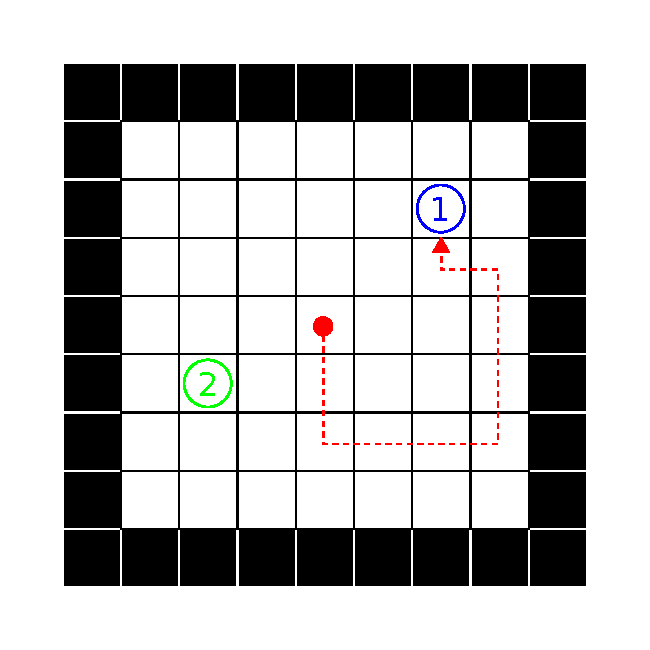
\includegraphics[keepaspectratio,width=\textwidth]{abbildungen/sample_not_seen.pdf}
    \subcaption{}
    \label{sample_visited}
  \end{subfigure}
  \begin{subfigure}[c]{0.5\textwidth}
    %\centering
    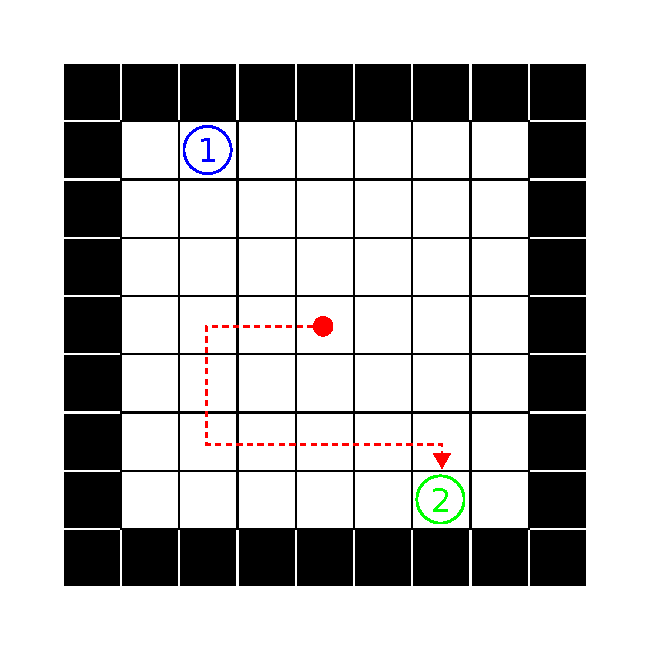
\includegraphics[keepaspectratio,width=\textwidth]{abbildungen/sample_visited.pdf}
    \subcaption{}
    \label{sample_visited}
  \end{subfigure}
  \begin{subfigure}[c]{0.5\textwidth}
    %\centering
    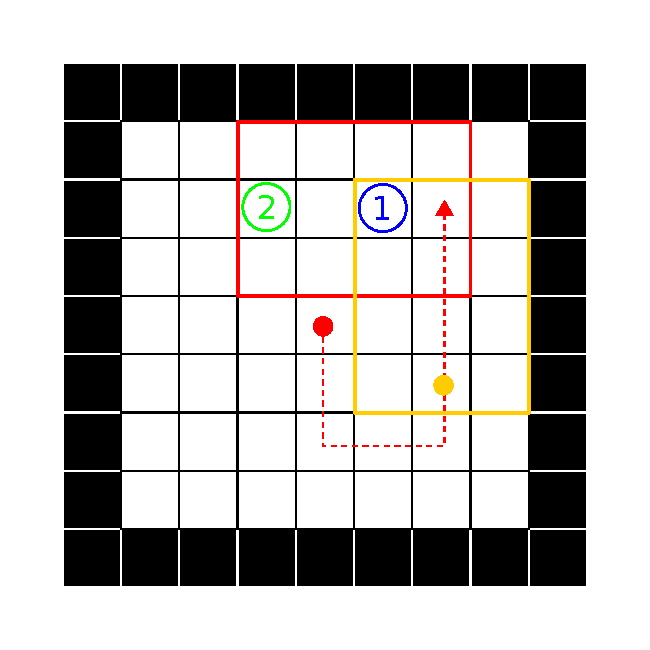
\includegraphics[keepaspectratio,width=\textwidth]{abbildungen/sample_seen.pdf}
    \subcaption{}
    \label{sample_seen2}
  \end{subfigure}
  \begin{subfigure}[c]{0.5\textwidth}
    %\centering
    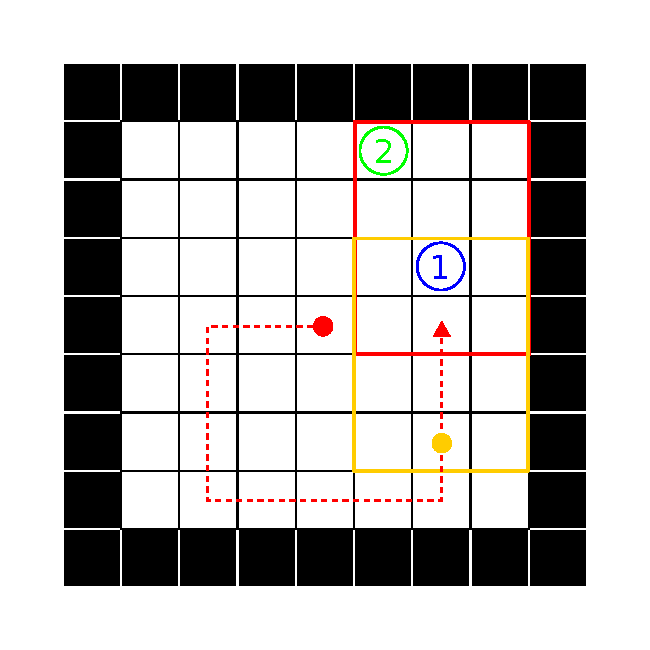
\includegraphics[keepaspectratio,width=\textwidth]{abbildungen/sample_seen2.pdf}
    \subcaption{}
    \label{sample_seen2}
  \end{subfigure}
  \caption{Blub}
\end{figure}
